\documentclass[12pt]{article}
\usepackage{tikz}
\usepackage{amsmath}
% Underlining package
\usepackage{ulem}
\usetikzlibrary{calc}
\usetikzlibrary{angles,quotes}
\usepackage[a4paper, portrait, margin=1cm]{geometry}
\usepackage{fancyhdr}

\newcommand{\HeadingAnswers}{%
\section*{\Large Name: \underline{\hspace{8cm}} \hfill Date: \underline{\hspace{3cm}}}%
\vspace{-3mm}\par
\textbf{Area Squares: Answers}\vspace{1pt}\hrule
}

% raise footer with page number; no header
\fancypagestyle{myfancypagestyle}{
  \fancyhf{}% clear all header and footer fields
  \renewcommand{\headrulewidth}{0pt} % no rule under header
  \fancyfoot[C] {\thepage} \setlength{\footskip}{14.5pt} % raise page number allowed min 14.5pt
}
\pagestyle{myfancypagestyle}  % apply myfancypagestyle

\newcounter{minipagecount}

\begin{document}
\HeadingAnswers
\vspace{8mm}

\begin{minipage}{0.55\textwidth}
  \refstepcounter{minipagecount}
  \noindent{(\theminipagecount)}\quad
  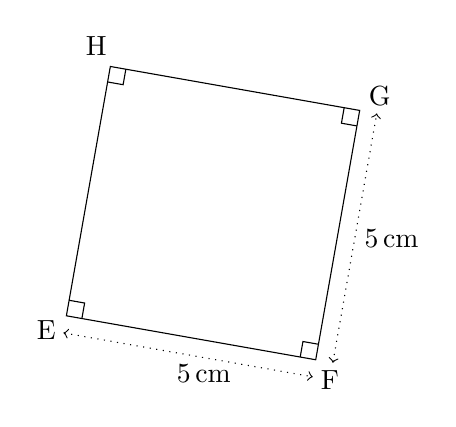
\begin{tikzpicture}[scale=1.1, baseline=(current bounding box.north)]
    \begin{scope}[rotate=-10]
        % Draw square
        \draw (0,0) coordinate (E) --
              ++(2.923,0) coordinate (F) --
              ++(0,2.923) coordinate (G) --
              ++(-2.923,0) coordinate (H) -- cycle;

        % Right angle markers
        \foreach \p/\q/\r in {H/E/F,E/F/G,F/G/H,G/H/E} {
            \pic [draw, -, angle radius=0.2cm] {right angle=\p--\q--\r};
        }

        % Vertex LABELS
        % Labels relative to shape geometry
        \node at ($(E)+(-0.2,-0.2)$) {E};
        \node at ($(F)+(0.2,-0.2)$) {F};
        \node at ($(G)+(0.2,0.2)$) {G};
        \node at ($(H)+(-0.2,0.2)$) {H};

        % Dotted arrows shifted away from edges
        % Horizontal side (A-B), shifted down
        \draw[<->, dotted]
            ($(E) + (0,-0.2cm)$) -- ($(F) + (0,-0.2cm)$)
            node[midway,below, xshift=2mm] {5\,cm};

        % Vertical side (B-C), shifted right
        \draw[<->, dotted]
            ($(F) + (0.2cm,0)$) -- ($(G) + (0.2cm,0)$)
            node[midway,right] {5\,cm};
    \end{scope}
\end{tikzpicture}
\end{minipage}%
\hfill
\begin{minipage}{.4\textwidth}
  \begin{align*}
  \text{Area} &= l^2 \\
  \text{Area} &= 5 \,\text{cm} \times 5 \,\text{cm} \\
  \text{Area} &= 25 \,\text{cm}^2
  \end{align*}
\end{minipage}
\par\vspace{1cm}\begin{minipage}{0.55\textwidth}
  \refstepcounter{minipagecount}
  \noindent{(\theminipagecount)}\quad
  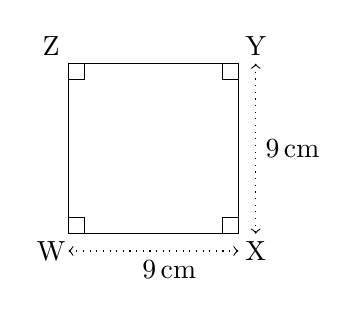
\begin{tikzpicture}[scale=1.1, baseline=(current bounding box.north)]
    \begin{scope}[rotate=0]
        % Draw square
        \draw (0,0) coordinate (W) --
              ++(1.962,0) coordinate (X) --
              ++(0,1.962) coordinate (Y) --
              ++(-1.962,0) coordinate (Z) -- cycle;

        % Right angle markers
        \foreach \p/\q/\r in {Z/W/X,W/X/Y,X/Y/Z,Y/Z/W} {
            \pic [draw, -, angle radius=0.2cm] {right angle=\p--\q--\r};
        }

        % Vertex LABELS
        % Labels relative to shape geometry
        \node at ($(W)+(-0.2,-0.2)$) {W};
        \node at ($(X)+(0.2,-0.2)$) {X};
        \node at ($(Y)+(0.2,0.2)$) {Y};
        \node at ($(Z)+(-0.2,0.2)$) {Z};

        % Dotted arrows shifted away from edges
        % Horizontal side (A-B), shifted down
        \draw[<->, dotted]
            ($(W) + (0,-0.2cm)$) -- ($(X) + (0,-0.2cm)$)
            node[midway,below, xshift=2mm] {9\,cm};

        % Vertical side (B-C), shifted right
        \draw[<->, dotted]
            ($(X) + (0.2cm,0)$) -- ($(Y) + (0.2cm,0)$)
            node[midway,right] {9\,cm};
    \end{scope}
\end{tikzpicture}
\end{minipage}%
\hfill
\begin{minipage}{.4\textwidth}
  \begin{align*}
  \text{Area} &= l^2 \\
  \text{Area} &= 9 \,\text{cm} \times 9 \,\text{cm} \\
  \text{Area} &= 81 \,\text{cm}^2
  \end{align*}
\end{minipage}
\par\vspace{1cm}\begin{minipage}{0.55\textwidth}
  \refstepcounter{minipagecount}
  \noindent{(\theminipagecount)}\quad
  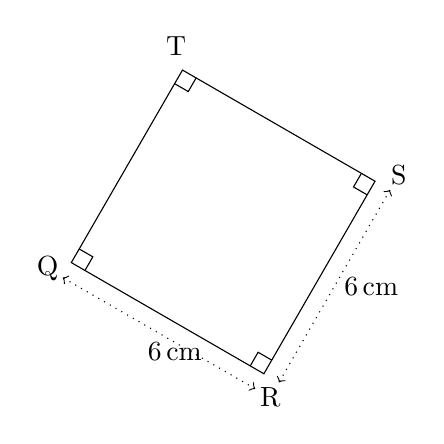
\begin{tikzpicture}[scale=1.1, baseline=(current bounding box.north)]
    \begin{scope}[rotate=-30]
        % Draw square
        \draw (0,0) coordinate (Q) --
              ++(2.567,0) coordinate (R) --
              ++(0,2.567) coordinate (S) --
              ++(-2.567,0) coordinate (T) -- cycle;

        % Right angle markers
        \foreach \p/\q/\r in {T/Q/R,Q/R/S,R/S/T,S/T/Q} {
            \pic [draw, -, angle radius=0.2cm] {right angle=\p--\q--\r};
        }

        % Vertex LABELS
        % Labels relative to shape geometry
        \node at ($(Q)+(-0.2,-0.2)$) {Q};
        \node at ($(R)+(0.2,-0.2)$) {R};
        \node at ($(S)+(0.2,0.2)$) {S};
        \node at ($(T)+(-0.2,0.2)$) {T};

        % Dotted arrows shifted away from edges
        % Horizontal side (A-B), shifted down
        \draw[<->, dotted]
            ($(Q) + (0,-0.2cm)$) -- ($(R) + (0,-0.2cm)$)
            node[midway,below, xshift=2mm] {6\,cm};

        % Vertical side (B-C), shifted right
        \draw[<->, dotted]
            ($(R) + (0.2cm,0)$) -- ($(S) + (0.2cm,0)$)
            node[midway,right] {6\,cm};
    \end{scope}
\end{tikzpicture}
\end{minipage}%
\hfill
\begin{minipage}{.4\textwidth}
  \begin{align*}
  \text{Area} &= l^2 \\
  \text{Area} &= 6 \,\text{cm} \times 6 \,\text{cm} \\
  \text{Area} &= 36 \,\text{cm}^2
  \end{align*}
\end{minipage}
\par\vspace{1cm}\begin{minipage}{0.55\textwidth}
  \refstepcounter{minipagecount}
  \noindent{(\theminipagecount)}\quad
  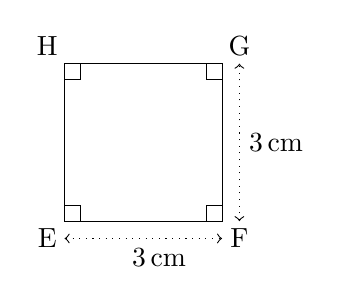
\begin{tikzpicture}[scale=1.1, baseline=(current bounding box.north)]
    \begin{scope}[rotate=0]
        % Draw square
        \draw (0,0) coordinate (E) --
              ++(1.818,0) coordinate (F) --
              ++(0,1.818) coordinate (G) --
              ++(-1.818,0) coordinate (H) -- cycle;

        % Right angle markers
        \foreach \p/\q/\r in {H/E/F,E/F/G,F/G/H,G/H/E} {
            \pic [draw, -, angle radius=0.2cm] {right angle=\p--\q--\r};
        }

        % Vertex LABELS
        % Labels relative to shape geometry
        \node at ($(E)+(-0.2,-0.2)$) {E};
        \node at ($(F)+(0.2,-0.2)$) {F};
        \node at ($(G)+(0.2,0.2)$) {G};
        \node at ($(H)+(-0.2,0.2)$) {H};

        % Dotted arrows shifted away from edges
        % Horizontal side (A-B), shifted down
        \draw[<->, dotted]
            ($(E) + (0,-0.2cm)$) -- ($(F) + (0,-0.2cm)$)
            node[midway,below, xshift=2mm] {3\,cm};

        % Vertical side (B-C), shifted right
        \draw[<->, dotted]
            ($(F) + (0.2cm,0)$) -- ($(G) + (0.2cm,0)$)
            node[midway,right] {3\,cm};
    \end{scope}
\end{tikzpicture}
\end{minipage}%
\hfill
\begin{minipage}{.4\textwidth}
  \begin{align*}
  \text{Area} &= l^2 \\
  \text{Area} &= 3 \,\text{cm} \times 3 \,\text{cm} \\
  \text{Area} &= 9 \,\text{cm}^2
  \end{align*}
\end{minipage}
\par\vspace{1cm}\begin{minipage}{0.55\textwidth}
  \refstepcounter{minipagecount}
  \noindent{(\theminipagecount)}\quad
  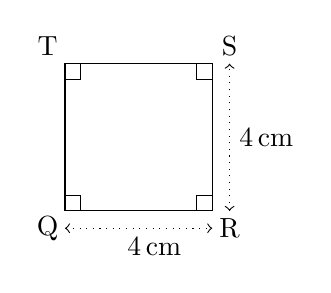
\begin{tikzpicture}[scale=1.1, baseline=(current bounding box.north)]
    \begin{scope}[rotate=0]
        % Draw square
        \draw (0,0) coordinate (Q) --
              ++(1.7,0) coordinate (R) --
              ++(0,1.7) coordinate (S) --
              ++(-1.7,0) coordinate (T) -- cycle;

        % Right angle markers
        \foreach \p/\q/\r in {T/Q/R,Q/R/S,R/S/T,S/T/Q} {
            \pic [draw, -, angle radius=0.2cm] {right angle=\p--\q--\r};
        }

        % Vertex LABELS
        % Labels relative to shape geometry
        \node at ($(Q)+(-0.2,-0.2)$) {Q};
        \node at ($(R)+(0.2,-0.2)$) {R};
        \node at ($(S)+(0.2,0.2)$) {S};
        \node at ($(T)+(-0.2,0.2)$) {T};

        % Dotted arrows shifted away from edges
        % Horizontal side (A-B), shifted down
        \draw[<->, dotted]
            ($(Q) + (0,-0.2cm)$) -- ($(R) + (0,-0.2cm)$)
            node[midway,below, xshift=2mm] {4\,cm};

        % Vertical side (B-C), shifted right
        \draw[<->, dotted]
            ($(R) + (0.2cm,0)$) -- ($(S) + (0.2cm,0)$)
            node[midway,right] {4\,cm};
    \end{scope}
\end{tikzpicture}
\end{minipage}%
\hfill
\begin{minipage}{.4\textwidth}
  \begin{align*}
  \text{Area} &= l^2 \\
  \text{Area} &= 4 \,\text{cm} \times 4 \,\text{cm} \\
  \text{Area} &= 16 \,\text{cm}^2
  \end{align*}
\end{minipage}
\par\vspace{1cm}\begin{minipage}{0.55\textwidth}
  \refstepcounter{minipagecount}
  \noindent{(\theminipagecount)}\quad
  \begin{tikzpicture}[scale=1.1, baseline=(current bounding box.north)]
    \begin{scope}[rotate=0]
        % Draw square
        \draw (0,0) coordinate (A) --
              ++(2.363,0) coordinate (B) --
              ++(0,2.363) coordinate (C) --
              ++(-2.363,0) coordinate (D) -- cycle;

        % Right angle markers
        \foreach \p/\q/\r in {D/A/B,A/B/C,B/C/D,C/D/A} {
            \pic [draw, -, angle radius=0.2cm] {right angle=\p--\q--\r};
        }

        % Vertex LABELS
        % Labels relative to shape geometry
        \node at ($(A)+(-0.2,-0.2)$) {A};
        \node at ($(B)+(0.2,-0.2)$) {B};
        \node at ($(C)+(0.2,0.2)$) {C};
        \node at ($(D)+(-0.2,0.2)$) {D};

        % Dotted arrows shifted away from edges
        % Horizontal side (A-B), shifted down
        \draw[<->, dotted]
            ($(A) + (0,-0.2cm)$) -- ($(B) + (0,-0.2cm)$)
            node[midway,below, xshift=2mm] {2\,cm};

        % Vertical side (B-C), shifted right
        \draw[<->, dotted]
            ($(B) + (0.2cm,0)$) -- ($(C) + (0.2cm,0)$)
            node[midway,right] {2\,cm};
    \end{scope}
\end{tikzpicture}
\end{minipage}%
\hfill
\begin{minipage}{.4\textwidth}
  \begin{align*}
  \text{Area} &= l^2 \\
  \text{Area} &= 2 \,\text{cm} \times 2 \,\text{cm} \\
  \text{Area} &= 4 \,\text{cm}^2
  \end{align*}
\end{minipage}
\par\vspace{1cm}\begin{minipage}{0.55\textwidth}
  \refstepcounter{minipagecount}
  \noindent{(\theminipagecount)}\quad
  \begin{tikzpicture}[scale=1.1, baseline=(current bounding box.north)]
    \begin{scope}[rotate=0]
        % Draw square
        \draw (0,0) coordinate (Q) --
              ++(2.813,0) coordinate (R) --
              ++(0,2.813) coordinate (S) --
              ++(-2.813,0) coordinate (T) -- cycle;

        % Right angle markers
        \foreach \p/\q/\r in {T/Q/R,Q/R/S,R/S/T,S/T/Q} {
            \pic [draw, -, angle radius=0.2cm] {right angle=\p--\q--\r};
        }

        % Vertex LABELS
        % Labels relative to shape geometry
        \node at ($(Q)+(-0.2,-0.2)$) {Q};
        \node at ($(R)+(0.2,-0.2)$) {R};
        \node at ($(S)+(0.2,0.2)$) {S};
        \node at ($(T)+(-0.2,0.2)$) {T};

        % Dotted arrows shifted away from edges
        % Horizontal side (A-B), shifted down
        \draw[<->, dotted]
            ($(Q) + (0,-0.2cm)$) -- ($(R) + (0,-0.2cm)$)
            node[midway,below, xshift=2mm] {7\,cm};

        % Vertical side (B-C), shifted right
        \draw[<->, dotted]
            ($(R) + (0.2cm,0)$) -- ($(S) + (0.2cm,0)$)
            node[midway,right] {7\,cm};
    \end{scope}
\end{tikzpicture}
\end{minipage}%
\hfill
\begin{minipage}{.4\textwidth}
  \begin{align*}
  \text{Area} &= l^2 \\
  \text{Area} &= 7 \,\text{cm} \times 7 \,\text{cm} \\
  \text{Area} &= 49 \,\text{cm}^2
  \end{align*}
\end{minipage}
\par\vspace{1cm}\begin{minipage}{0.55\textwidth}
  \refstepcounter{minipagecount}
  \noindent{(\theminipagecount)}\quad
  \begin{tikzpicture}[scale=1.1, baseline=(current bounding box.north)]
    \begin{scope}[rotate=0]
        % Draw square
        \draw (0,0) coordinate (W) --
              ++(2.655,0) coordinate (X) --
              ++(0,2.655) coordinate (Y) --
              ++(-2.655,0) coordinate (Z) -- cycle;

        % Right angle markers
        \foreach \p/\q/\r in {Z/W/X,W/X/Y,X/Y/Z,Y/Z/W} {
            \pic [draw, -, angle radius=0.2cm] {right angle=\p--\q--\r};
        }

        % Vertex LABELS
        % Labels relative to shape geometry
        \node at ($(W)+(-0.2,-0.2)$) {W};
        \node at ($(X)+(0.2,-0.2)$) {X};
        \node at ($(Y)+(0.2,0.2)$) {Y};
        \node at ($(Z)+(-0.2,0.2)$) {Z};

        % Dotted arrows shifted away from edges
        % Horizontal side (A-B), shifted down
        \draw[<->, dotted]
            ($(W) + (0,-0.2cm)$) -- ($(X) + (0,-0.2cm)$)
            node[midway,below, xshift=2mm] {1\,cm};

        % Vertical side (B-C), shifted right
        \draw[<->, dotted]
            ($(X) + (0.2cm,0)$) -- ($(Y) + (0.2cm,0)$)
            node[midway,right] {1\,cm};
    \end{scope}
\end{tikzpicture}
\end{minipage}%
\hfill
\begin{minipage}{.4\textwidth}
  \begin{align*}
  \text{Area} &= l^2 \\
  \text{Area} &= 1 \,\text{cm} \times 1 \,\text{cm} \\
  \text{Area} &= 1 \,\text{cm}^2
  \end{align*}
\end{minipage}
\par\vspace{1cm}\begin{minipage}{0.55\textwidth}
  \refstepcounter{minipagecount}
  \noindent{(\theminipagecount)}\quad
  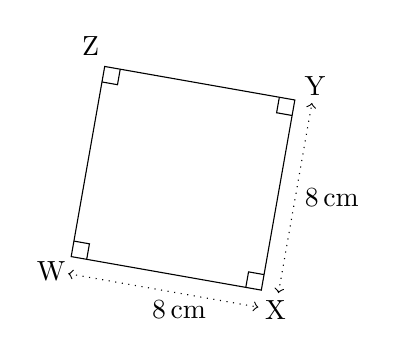
\begin{tikzpicture}[scale=1.1, baseline=(current bounding box.north)]
    \begin{scope}[rotate=-10]
        % Draw square
        \draw (0,0) coordinate (W) --
              ++(2.229,0) coordinate (X) --
              ++(0,2.229) coordinate (Y) --
              ++(-2.229,0) coordinate (Z) -- cycle;

        % Right angle markers
        \foreach \p/\q/\r in {Z/W/X,W/X/Y,X/Y/Z,Y/Z/W} {
            \pic [draw, -, angle radius=0.2cm] {right angle=\p--\q--\r};
        }

        % Vertex LABELS
        % Labels relative to shape geometry
        \node at ($(W)+(-0.2,-0.2)$) {W};
        \node at ($(X)+(0.2,-0.2)$) {X};
        \node at ($(Y)+(0.2,0.2)$) {Y};
        \node at ($(Z)+(-0.2,0.2)$) {Z};

        % Dotted arrows shifted away from edges
        % Horizontal side (A-B), shifted down
        \draw[<->, dotted]
            ($(W) + (0,-0.2cm)$) -- ($(X) + (0,-0.2cm)$)
            node[midway,below, xshift=2mm] {8\,cm};

        % Vertical side (B-C), shifted right
        \draw[<->, dotted]
            ($(X) + (0.2cm,0)$) -- ($(Y) + (0.2cm,0)$)
            node[midway,right] {8\,cm};
    \end{scope}
\end{tikzpicture}
\end{minipage}%
\hfill
\begin{minipage}{.4\textwidth}
  \begin{align*}
  \text{Area} &= l^2 \\
  \text{Area} &= 8 \,\text{cm} \times 8 \,\text{cm} \\
  \text{Area} &= 64 \,\text{cm}^2
  \end{align*}
\end{minipage}
\par\vspace{1cm}\begin{minipage}{0.55\textwidth}
  \refstepcounter{minipagecount}
  \noindent{(\theminipagecount)}\quad
  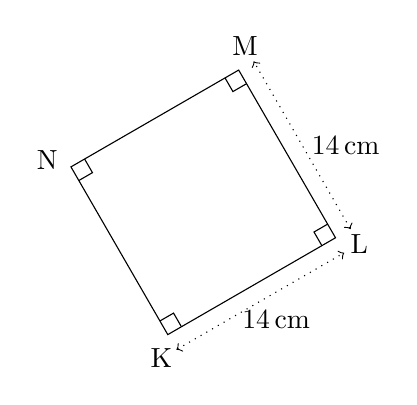
\begin{tikzpicture}[scale=1.1, baseline=(current bounding box.north)]
    \begin{scope}[rotate=30]
        % Draw square
        \draw (0,0) coordinate (K) --
              ++(2.236,0) coordinate (L) --
              ++(0,2.236) coordinate (M) --
              ++(-2.236,0) coordinate (N) -- cycle;

        % Right angle markers
        \foreach \p/\q/\r in {N/K/L,K/L/M,L/M/N,M/N/K} {
            \pic [draw, -, angle radius=0.2cm] {right angle=\p--\q--\r};
        }

        % Vertex LABELS
        % Labels relative to shape geometry
        \node at ($(K)+(-0.2,-0.2)$) {K};
        \node at ($(L)+(0.2,-0.2)$) {L};
        \node at ($(M)+(0.2,0.2)$) {M};
        \node at ($(N)+(-0.2,0.2)$) {N};

        % Dotted arrows shifted away from edges
        % Horizontal side (A-B), shifted down
        \draw[<->, dotted]
            ($(K) + (0,-0.2cm)$) -- ($(L) + (0,-0.2cm)$)
            node[midway,below, xshift=2mm] {14\,cm};

        % Vertical side (B-C), shifted right
        \draw[<->, dotted]
            ($(L) + (0.2cm,0)$) -- ($(M) + (0.2cm,0)$)
            node[midway,right] {14\,cm};
    \end{scope}
\end{tikzpicture}
\end{minipage}%
\hfill
\begin{minipage}{.4\textwidth}
  \begin{align*}
  \text{Area} &= l^2 \\
  \text{Area} &= 14 \,\text{cm} \times 14 \,\text{cm} \\
  \text{Area} &= 196 \,\text{cm}^2
  \end{align*}
\end{minipage}
\par\vspace{1cm}\begin{minipage}{0.55\textwidth}
  \refstepcounter{minipagecount}
  \noindent{(\theminipagecount)}\quad
  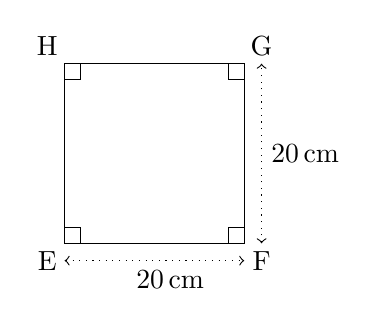
\begin{tikzpicture}[scale=1.1, baseline=(current bounding box.north)]
    \begin{scope}[rotate=0]
        % Draw square
        \draw (0,0) coordinate (E) --
              ++(2.074,0) coordinate (F) --
              ++(0,2.074) coordinate (G) --
              ++(-2.074,0) coordinate (H) -- cycle;

        % Right angle markers
        \foreach \p/\q/\r in {H/E/F,E/F/G,F/G/H,G/H/E} {
            \pic [draw, -, angle radius=0.2cm] {right angle=\p--\q--\r};
        }

        % Vertex LABELS
        % Labels relative to shape geometry
        \node at ($(E)+(-0.2,-0.2)$) {E};
        \node at ($(F)+(0.2,-0.2)$) {F};
        \node at ($(G)+(0.2,0.2)$) {G};
        \node at ($(H)+(-0.2,0.2)$) {H};

        % Dotted arrows shifted away from edges
        % Horizontal side (A-B), shifted down
        \draw[<->, dotted]
            ($(E) + (0,-0.2cm)$) -- ($(F) + (0,-0.2cm)$)
            node[midway,below, xshift=2mm] {20\,cm};

        % Vertical side (B-C), shifted right
        \draw[<->, dotted]
            ($(F) + (0.2cm,0)$) -- ($(G) + (0.2cm,0)$)
            node[midway,right] {20\,cm};
    \end{scope}
\end{tikzpicture}
\end{minipage}%
\hfill
\begin{minipage}{.4\textwidth}
  \begin{align*}
  \text{Area} &= l^2 \\
  \text{Area} &= 20 \,\text{cm} \times 20 \,\text{cm} \\
  \text{Area} &= 400 \,\text{cm}^2
  \end{align*}
\end{minipage}
\par\vspace{1cm}\begin{minipage}{0.55\textwidth}
  \refstepcounter{minipagecount}
  \noindent{(\theminipagecount)}\quad
  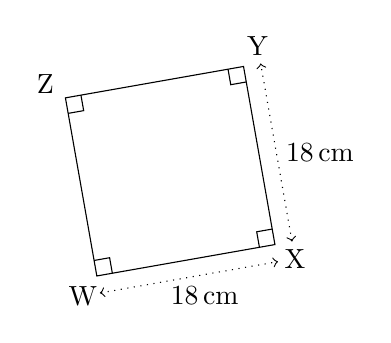
\begin{tikzpicture}[scale=1.1, baseline=(current bounding box.north)]
    \begin{scope}[rotate=10]
        % Draw square
        \draw (0,0) coordinate (W) --
              ++(2.088,0) coordinate (X) --
              ++(0,2.088) coordinate (Y) --
              ++(-2.088,0) coordinate (Z) -- cycle;

        % Right angle markers
        \foreach \p/\q/\r in {Z/W/X,W/X/Y,X/Y/Z,Y/Z/W} {
            \pic [draw, -, angle radius=0.2cm] {right angle=\p--\q--\r};
        }

        % Vertex LABELS
        % Labels relative to shape geometry
        \node at ($(W)+(-0.2,-0.2)$) {W};
        \node at ($(X)+(0.2,-0.2)$) {X};
        \node at ($(Y)+(0.2,0.2)$) {Y};
        \node at ($(Z)+(-0.2,0.2)$) {Z};

        % Dotted arrows shifted away from edges
        % Horizontal side (A-B), shifted down
        \draw[<->, dotted]
            ($(W) + (0,-0.2cm)$) -- ($(X) + (0,-0.2cm)$)
            node[midway,below, xshift=2mm] {18\,cm};

        % Vertical side (B-C), shifted right
        \draw[<->, dotted]
            ($(X) + (0.2cm,0)$) -- ($(Y) + (0.2cm,0)$)
            node[midway,right] {18\,cm};
    \end{scope}
\end{tikzpicture}
\end{minipage}%
\hfill
\begin{minipage}{.4\textwidth}
  \begin{align*}
  \text{Area} &= l^2 \\
  \text{Area} &= 18 \,\text{cm} \times 18 \,\text{cm} \\
  \text{Area} &= 324 \,\text{cm}^2
  \end{align*}
\end{minipage}
\par\vspace{1cm}\begin{minipage}{0.55\textwidth}
  \refstepcounter{minipagecount}
  \noindent{(\theminipagecount)}\quad
  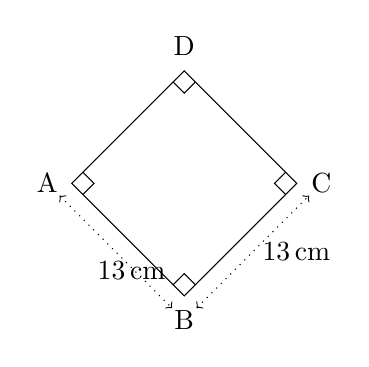
\begin{tikzpicture}[scale=1.1, baseline=(current bounding box.north)]
    \begin{scope}[rotate=-45]
        % Draw square
        \draw (0,0) coordinate (A) --
              ++(1.837,0) coordinate (B) --
              ++(0,1.837) coordinate (C) --
              ++(-1.837,0) coordinate (D) -- cycle;

        % Right angle markers
        \foreach \p/\q/\r in {D/A/B,A/B/C,B/C/D,C/D/A} {
            \pic [draw, -, angle radius=0.2cm] {right angle=\p--\q--\r};
        }

        % Vertex LABELS
        % Labels relative to shape geometry
        \node at ($(A)+(-0.2,-0.2)$) {A};
        \node at ($(B)+(0.2,-0.2)$) {B};
        \node at ($(C)+(0.2,0.2)$) {C};
        \node at ($(D)+(-0.2,0.2)$) {D};

        % Dotted arrows shifted away from edges
        % Horizontal side (A-B), shifted down
        \draw[<->, dotted]
            ($(A) + (0,-0.2cm)$) -- ($(B) + (0,-0.2cm)$)
            node[midway,below, xshift=2mm] {13\,cm};

        % Vertical side (B-C), shifted right
        \draw[<->, dotted]
            ($(B) + (0.2cm,0)$) -- ($(C) + (0.2cm,0)$)
            node[midway,right] {13\,cm};
    \end{scope}
\end{tikzpicture}
\end{minipage}%
\hfill
\begin{minipage}{.4\textwidth}
  \begin{align*}
  \text{Area} &= l^2 \\
  \text{Area} &= 13 \,\text{cm} \times 13 \,\text{cm} \\
  \text{Area} &= 169 \,\text{cm}^2
  \end{align*}
\end{minipage}
\par\vspace{1cm}\begin{minipage}{0.55\textwidth}
  \refstepcounter{minipagecount}
  \noindent{(\theminipagecount)}\quad
  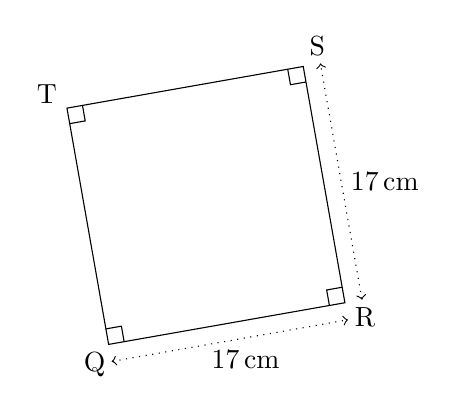
\begin{tikzpicture}[scale=1.1, baseline=(current bounding box.north)]
    \begin{scope}[rotate=10]
        % Draw square
        \draw (0,0) coordinate (Q) --
              ++(2.77,0) coordinate (R) --
              ++(0,2.77) coordinate (S) --
              ++(-2.77,0) coordinate (T) -- cycle;

        % Right angle markers
        \foreach \p/\q/\r in {T/Q/R,Q/R/S,R/S/T,S/T/Q} {
            \pic [draw, -, angle radius=0.2cm] {right angle=\p--\q--\r};
        }

        % Vertex LABELS
        % Labels relative to shape geometry
        \node at ($(Q)+(-0.2,-0.2)$) {Q};
        \node at ($(R)+(0.2,-0.2)$) {R};
        \node at ($(S)+(0.2,0.2)$) {S};
        \node at ($(T)+(-0.2,0.2)$) {T};

        % Dotted arrows shifted away from edges
        % Horizontal side (A-B), shifted down
        \draw[<->, dotted]
            ($(Q) + (0,-0.2cm)$) -- ($(R) + (0,-0.2cm)$)
            node[midway,below, xshift=2mm] {17\,cm};

        % Vertical side (B-C), shifted right
        \draw[<->, dotted]
            ($(R) + (0.2cm,0)$) -- ($(S) + (0.2cm,0)$)
            node[midway,right] {17\,cm};
    \end{scope}
\end{tikzpicture}
\end{minipage}%
\hfill
\begin{minipage}{.4\textwidth}
  \begin{align*}
  \text{Area} &= l^2 \\
  \text{Area} &= 17 \,\text{cm} \times 17 \,\text{cm} \\
  \text{Area} &= 289 \,\text{cm}^2
  \end{align*}
\end{minipage}
\par\vspace{1cm}\begin{minipage}{0.55\textwidth}
  \refstepcounter{minipagecount}
  \noindent{(\theminipagecount)}\quad
  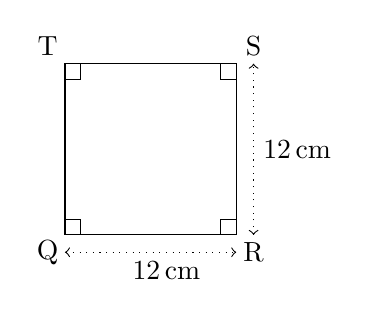
\begin{tikzpicture}[scale=1.1, baseline=(current bounding box.north)]
    \begin{scope}[rotate=0]
        % Draw square
        \draw (0,0) coordinate (Q) --
              ++(1.977,0) coordinate (R) --
              ++(0,1.977) coordinate (S) --
              ++(-1.977,0) coordinate (T) -- cycle;

        % Right angle markers
        \foreach \p/\q/\r in {T/Q/R,Q/R/S,R/S/T,S/T/Q} {
            \pic [draw, -, angle radius=0.2cm] {right angle=\p--\q--\r};
        }

        % Vertex LABELS
        % Labels relative to shape geometry
        \node at ($(Q)+(-0.2,-0.2)$) {Q};
        \node at ($(R)+(0.2,-0.2)$) {R};
        \node at ($(S)+(0.2,0.2)$) {S};
        \node at ($(T)+(-0.2,0.2)$) {T};

        % Dotted arrows shifted away from edges
        % Horizontal side (A-B), shifted down
        \draw[<->, dotted]
            ($(Q) + (0,-0.2cm)$) -- ($(R) + (0,-0.2cm)$)
            node[midway,below, xshift=2mm] {12\,cm};

        % Vertical side (B-C), shifted right
        \draw[<->, dotted]
            ($(R) + (0.2cm,0)$) -- ($(S) + (0.2cm,0)$)
            node[midway,right] {12\,cm};
    \end{scope}
\end{tikzpicture}
\end{minipage}%
\hfill
\begin{minipage}{.4\textwidth}
  \begin{align*}
  \text{Area} &= l^2 \\
  \text{Area} &= 12 \,\text{cm} \times 12 \,\text{cm} \\
  \text{Area} &= 144 \,\text{cm}^2
  \end{align*}
\end{minipage}
\par\vspace{1cm}\begin{minipage}{0.55\textwidth}
  \refstepcounter{minipagecount}
  \noindent{(\theminipagecount)}\quad
  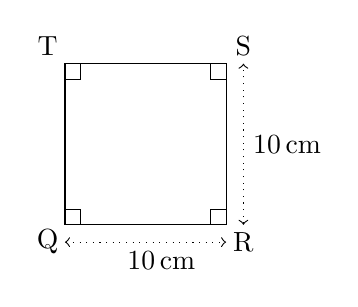
\begin{tikzpicture}[scale=1.1, baseline=(current bounding box.north)]
    \begin{scope}[rotate=0]
        % Draw square
        \draw (0,0) coordinate (Q) --
              ++(1.86,0) coordinate (R) --
              ++(0,1.86) coordinate (S) --
              ++(-1.86,0) coordinate (T) -- cycle;

        % Right angle markers
        \foreach \p/\q/\r in {T/Q/R,Q/R/S,R/S/T,S/T/Q} {
            \pic [draw, -, angle radius=0.2cm] {right angle=\p--\q--\r};
        }

        % Vertex LABELS
        % Labels relative to shape geometry
        \node at ($(Q)+(-0.2,-0.2)$) {Q};
        \node at ($(R)+(0.2,-0.2)$) {R};
        \node at ($(S)+(0.2,0.2)$) {S};
        \node at ($(T)+(-0.2,0.2)$) {T};

        % Dotted arrows shifted away from edges
        % Horizontal side (A-B), shifted down
        \draw[<->, dotted]
            ($(Q) + (0,-0.2cm)$) -- ($(R) + (0,-0.2cm)$)
            node[midway,below, xshift=2mm] {10\,cm};

        % Vertical side (B-C), shifted right
        \draw[<->, dotted]
            ($(R) + (0.2cm,0)$) -- ($(S) + (0.2cm,0)$)
            node[midway,right] {10\,cm};
    \end{scope}
\end{tikzpicture}
\end{minipage}%
\hfill
\begin{minipage}{.4\textwidth}
  \begin{align*}
  \text{Area} &= l^2 \\
  \text{Area} &= 10 \,\text{cm} \times 10 \,\text{cm} \\
  \text{Area} &= 100 \,\text{cm}^2
  \end{align*}
\end{minipage}
\par\vspace{1cm}\begin{minipage}{0.55\textwidth}
  \refstepcounter{minipagecount}
  \noindent{(\theminipagecount)}\quad
  \begin{tikzpicture}[scale=1.1, baseline=(current bounding box.north)]
    \begin{scope}[rotate=0]
        % Draw square
        \draw (0,0) coordinate (Q) --
              ++(2.962,0) coordinate (R) --
              ++(0,2.962) coordinate (S) --
              ++(-2.962,0) coordinate (T) -- cycle;

        % Right angle markers
        \foreach \p/\q/\r in {T/Q/R,Q/R/S,R/S/T,S/T/Q} {
            \pic [draw, -, angle radius=0.2cm] {right angle=\p--\q--\r};
        }

        % Vertex LABELS
        % Labels relative to shape geometry
        \node at ($(Q)+(-0.2,-0.2)$) {Q};
        \node at ($(R)+(0.2,-0.2)$) {R};
        \node at ($(S)+(0.2,0.2)$) {S};
        \node at ($(T)+(-0.2,0.2)$) {T};

        % Dotted arrows shifted away from edges
        % Horizontal side (A-B), shifted down
        \draw[<->, dotted]
            ($(Q) + (0,-0.2cm)$) -- ($(R) + (0,-0.2cm)$)
            node[midway,below, xshift=2mm] {11\,cm};

        % Vertical side (B-C), shifted right
        \draw[<->, dotted]
            ($(R) + (0.2cm,0)$) -- ($(S) + (0.2cm,0)$)
            node[midway,right] {11\,cm};
    \end{scope}
\end{tikzpicture}
\end{minipage}%
\hfill
\begin{minipage}{.4\textwidth}
  \begin{align*}
  \text{Area} &= l^2 \\
  \text{Area} &= 11 \,\text{cm} \times 11 \,\text{cm} \\
  \text{Area} &= 121 \,\text{cm}^2
  \end{align*}
\end{minipage}
\par\vspace{1cm}\begin{minipage}{0.55\textwidth}
  \refstepcounter{minipagecount}
  \noindent{(\theminipagecount)}\quad
  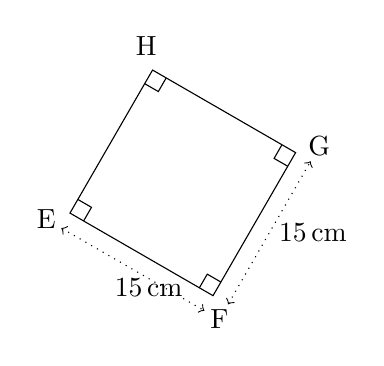
\begin{tikzpicture}[scale=1.1, baseline=(current bounding box.north)]
    \begin{scope}[rotate=-30]
        % Draw square
        \draw (0,0) coordinate (E) --
              ++(1.907,0) coordinate (F) --
              ++(0,1.907) coordinate (G) --
              ++(-1.907,0) coordinate (H) -- cycle;

        % Right angle markers
        \foreach \p/\q/\r in {H/E/F,E/F/G,F/G/H,G/H/E} {
            \pic [draw, -, angle radius=0.2cm] {right angle=\p--\q--\r};
        }

        % Vertex LABELS
        % Labels relative to shape geometry
        \node at ($(E)+(-0.2,-0.2)$) {E};
        \node at ($(F)+(0.2,-0.2)$) {F};
        \node at ($(G)+(0.2,0.2)$) {G};
        \node at ($(H)+(-0.2,0.2)$) {H};

        % Dotted arrows shifted away from edges
        % Horizontal side (A-B), shifted down
        \draw[<->, dotted]
            ($(E) + (0,-0.2cm)$) -- ($(F) + (0,-0.2cm)$)
            node[midway,below, xshift=2mm] {15\,cm};

        % Vertical side (B-C), shifted right
        \draw[<->, dotted]
            ($(F) + (0.2cm,0)$) -- ($(G) + (0.2cm,0)$)
            node[midway,right] {15\,cm};
    \end{scope}
\end{tikzpicture}
\end{minipage}%
\hfill
\begin{minipage}{.4\textwidth}
  \begin{align*}
  \text{Area} &= l^2 \\
  \text{Area} &= 15 \,\text{cm} \times 15 \,\text{cm} \\
  \text{Area} &= 225 \,\text{cm}^2
  \end{align*}
\end{minipage}
\par\vspace{1cm}\begin{minipage}{0.55\textwidth}
  \refstepcounter{minipagecount}
  \noindent{(\theminipagecount)}\quad
  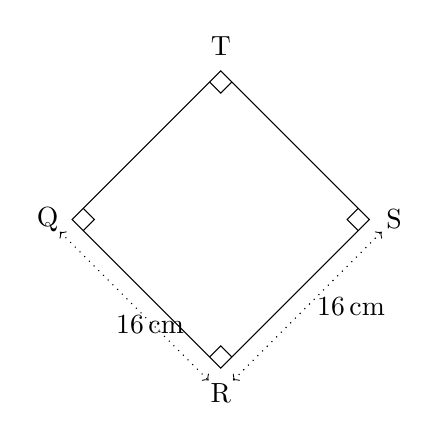
\begin{tikzpicture}[scale=1.1, baseline=(current bounding box.north)]
    \begin{scope}[rotate=-45]
        % Draw square
        \draw (0,0) coordinate (Q) --
              ++(2.427,0) coordinate (R) --
              ++(0,2.427) coordinate (S) --
              ++(-2.427,0) coordinate (T) -- cycle;

        % Right angle markers
        \foreach \p/\q/\r in {T/Q/R,Q/R/S,R/S/T,S/T/Q} {
            \pic [draw, -, angle radius=0.2cm] {right angle=\p--\q--\r};
        }

        % Vertex LABELS
        % Labels relative to shape geometry
        \node at ($(Q)+(-0.2,-0.2)$) {Q};
        \node at ($(R)+(0.2,-0.2)$) {R};
        \node at ($(S)+(0.2,0.2)$) {S};
        \node at ($(T)+(-0.2,0.2)$) {T};

        % Dotted arrows shifted away from edges
        % Horizontal side (A-B), shifted down
        \draw[<->, dotted]
            ($(Q) + (0,-0.2cm)$) -- ($(R) + (0,-0.2cm)$)
            node[midway,below, xshift=2mm] {16\,cm};

        % Vertical side (B-C), shifted right
        \draw[<->, dotted]
            ($(R) + (0.2cm,0)$) -- ($(S) + (0.2cm,0)$)
            node[midway,right] {16\,cm};
    \end{scope}
\end{tikzpicture}
\end{minipage}%
\hfill
\begin{minipage}{.4\textwidth}
  \begin{align*}
  \text{Area} &= l^2 \\
  \text{Area} &= 16 \,\text{cm} \times 16 \,\text{cm} \\
  \text{Area} &= 256 \,\text{cm}^2
  \end{align*}
\end{minipage}
\par\vspace{1cm}\begin{minipage}{0.55\textwidth}
  \refstepcounter{minipagecount}
  \noindent{(\theminipagecount)}\quad
  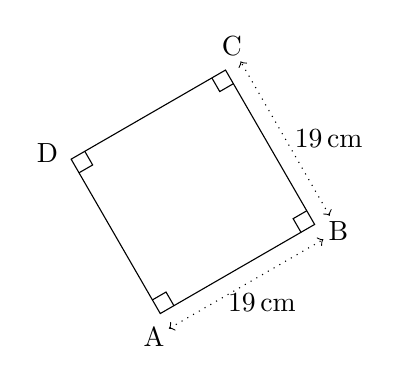
\begin{tikzpicture}[scale=1.1, baseline=(current bounding box.north)]
    \begin{scope}[rotate=30]
        % Draw square
        \draw (0,0) coordinate (A) --
              ++(2.058,0) coordinate (B) --
              ++(0,2.058) coordinate (C) --
              ++(-2.058,0) coordinate (D) -- cycle;

        % Right angle markers
        \foreach \p/\q/\r in {D/A/B,A/B/C,B/C/D,C/D/A} {
            \pic [draw, -, angle radius=0.2cm] {right angle=\p--\q--\r};
        }

        % Vertex LABELS
        % Labels relative to shape geometry
        \node at ($(A)+(-0.2,-0.2)$) {A};
        \node at ($(B)+(0.2,-0.2)$) {B};
        \node at ($(C)+(0.2,0.2)$) {C};
        \node at ($(D)+(-0.2,0.2)$) {D};

        % Dotted arrows shifted away from edges
        % Horizontal side (A-B), shifted down
        \draw[<->, dotted]
            ($(A) + (0,-0.2cm)$) -- ($(B) + (0,-0.2cm)$)
            node[midway,below, xshift=2mm] {19\,cm};

        % Vertical side (B-C), shifted right
        \draw[<->, dotted]
            ($(B) + (0.2cm,0)$) -- ($(C) + (0.2cm,0)$)
            node[midway,right] {19\,cm};
    \end{scope}
\end{tikzpicture}
\end{minipage}%
\hfill
\begin{minipage}{.4\textwidth}
  \begin{align*}
  \text{Area} &= l^2 \\
  \text{Area} &= 19 \,\text{cm} \times 19 \,\text{cm} \\
  \text{Area} &= 361 \,\text{cm}^2
  \end{align*}
\end{minipage}
\par\vspace{1cm}

\end{document}
